\documentclass[aspectratio=169]{beamer}

% ===================== PACKAGES =====================
\usepackage[utf8]{inputenc}
\usepackage{amsmath,amssymb}
\usepackage{tikz}
\usetikzlibrary{positioning,shapes,arrows.meta}
\usepackage{booktabs}
\usepackage{array}

% ===================== THEME =====================
\usetheme{Madrid}
\usecolortheme{beaver}
\setbeamertemplate{navigation symbols}{}
\setbeamertemplate{footline}[frame number]

\title[Sets \& Set Theory]{Mathematics of Computing}
\subtitle{Sets: Set-Builder Form, Types, Operations \& Hasse Diagrams}
\author{Aishwarya J S}
\date{\today}

% ===================== TIKZ HELPERS =====================
% Two overlapping circles, radius r, centers (0,0) and (d,0)
\newcommand{\circA}{(0,0) circle (1.3)}
\newcommand{\circB}{(1.3,0) circle (1.3)}

\begin{document}

% ---------------------------------------------------------
\begin{frame}
\titlepage
\end{frame}

\begin{frame}{Outline}
\tableofcontents
\end{frame}

% ===========================================================
\section{Ten Sets and Set-Builder Form}
% ===========================================================

\begin{frame}{Sets and Set-Builder Form (1--3)}
\small
\begin{enumerate}
\item $S=\{-5,-3,-1,1,3,5\}$ \\
$S=\{x \mid x\in \mathbb{Z},\ x \text{ is odd},\ -5\le x \le 5\}$

\bigskip
\item $S=\left\{\dfrac{1}{2},\dfrac{1}{3},\dfrac{1}{4},\dfrac{1}{5},\dfrac{1}{6}\right\}$ \\
$S=\left\{\dfrac{1}{x} \;\middle|\; x\in \mathbb{Z},\ 2\le x \le 6\right\}$

\bigskip
\item $S=\{1,3,6,10,15,21,\dots\}$ \quad (triangular numbers) \\
$S=\left\{x \;\middle|\; x=\dfrac{n(n+1)}{2},\ n\in \mathbb{N}\right\}$
\end{enumerate}
\end{frame}

\begin{frame}{Sets and Set-Builder Form (4--6)}
\small
\begin{enumerate}
\setcounter{enumi}{3}
\item $S=\{\dots,-10,-5,0,5,10,\dots\}$ \\
$S=\{x \mid 5 \mid x,\ x\in \mathbb{Z}\}$

\bigskip
\item $S=\{1,5,9,13,17,\dots\}$ \\
$S=\{x \mid x \equiv 1 \pmod{4},\ x\in \mathbb{N}\}$ \\


\bigskip
\item $S=\left\{1,-1,\dfrac{1}{2},-\dfrac{1}{2},\dfrac{1}{3},-\dfrac{1}{3},\dots\right\}$ \\
$S=\left\{x \;\middle|\; x=\dfrac{(-1)^n}{n},\ n\in \mathbb{N}\right\}$
\end{enumerate}
\end{frame}

\begin{frame}{Sets and Set-Builder Form (7--10)}
\small
\begin{enumerate}
\setcounter{enumi}{6}
\item $S=\{0,\pm 1,\pm 4,\pm 9,\pm 16,\dots\}$ \\
$S=\{x \mid x=(-1)^n\, n^2,\ n\in \mathbb{W}\}$ \quad {\footnotesize ($\mathbb{W}=$ whole numbers)}

\bigskip
\item \textbf{Mersenne numbers:} $M=\{1,3,7,15,31,63,\dots\}$ \\
$M=\{x \mid x=2^n-1,\ n\in \mathbb{N}\}$

\bigskip
\item $S=\{(1,9),(2,8),(3,7),(4,6),(5,5),\dots\}$ \\
$S=\{(x,y) \mid x+y=10,\ (x,y)\in \mathbb{N}\times\mathbb{N}\}$

\bigskip
\item $S=\{(1,1),(2,8),(3,3),(4,4),(8,8),\dots\}$ \\
$S=\{(x,y) \mid (x,y)\in \mathbb{N}\times\mathbb{N},\ xy=n^2,\ n\in \mathbb{N}\}$
\end{enumerate}
\end{frame}

% ===========================================================
\section{Types of Sets}
% ===========================================================

\begin{frame}{Types of Sets: Cardinality}
\begin{block}{Definition}
The \textbf{cardinality} of a set is the number of distinct elements in it, denoted $|A|$ or $n(A)$.
\end{block}
\begin{exampleblock}{Example}
$A=\{2,4,6,8\} \implies |A|=4$ \\
$A=\{a_1,a_2,\dots,a_n\} \implies |A|=n$
\end{exampleblock}
\begin{exampleblock}{ML/AI Examples}
\begin{itemize}
\item Feature set: $F=\{\text{Age, BMI, Glucose, Blood Pressure, Insulin}\}$, $|F|=5$
\item NLP vocabulary: $V=\{w_1,w_2,\dots,w_{50000}\}$, $|V|=50000$
\end{itemize}
\end{exampleblock}
\end{frame}

\begin{frame}{Finite and Infinite Sets}
\begin{columns}
\column{0.5\textwidth}
\begin{block}{Finite Set}
Contains a finite number of elements; there exists $n\in\mathbb{N}_0$ such that $|A|=n$.
\end{block}
\begin{exampleblock}{Example}
Feature set $F=\{\text{Age,BMI,Glucose,BP,Insulin}\}$, $|F|=5$
\end{exampleblock}

\column{0.5\textwidth}
\begin{block}{Infinite Set}
Cardinality is infinite ($|A|=\infty$).
\end{block}
\begin{exampleblock}{Examples}
Feature space $X=\mathbb{R}^3$ (age, height, weight) $\Rightarrow |X|=\infty$ \\
Weight space $W=\mathbb{R}^n$ of a neural network $\Rightarrow |W|=\infty$
\end{exampleblock}
\end{columns}
\end{frame}

\begin{frame}{Null (Empty) Set}
\begin{block}{Definition}
A set that contains no elements. $A=\{\}$ or $\varnothing$, $|A|=0$.
\end{block}
\begin{exampleblock}{Examples}
\textbf{ML dataset query:} \\
$D=\{x\in \text{Training Dataset} \mid \text{Age}<0\} = \varnothing$

\medskip
\textbf{Computer Vision:} \\
$C=\{x\in \text{Image Dataset} \mid x \text{ is both a cat and a car}\} = \varnothing$
\end{exampleblock}
\end{frame}

\begin{frame}{Equal Sets}
\begin{block}{Definition}
Two sets are \textbf{equal} if they contain exactly the same elements, irrespective of order:
$$A=B \iff \forall x\,(x\in A \iff x\in B) \iff A\subseteq B \text{ and } B\subseteq A$$
\end{block}
\begin{exampleblock}{Example: Graph Neural Networks -- Edge Set}
Suppose a graph is represented as:
$$E_1=\{(v_1,v_2),(v_2,v_3),(v_3,v_4)\}, \qquad E_2=\{(v_3,v_4),(v_1,v_2),(v_2,v_3)\}$$
Since both sets contain exactly the same edges: $E_1=E_2$.
\end{exampleblock}
\end{frame}

\begin{frame}{Equivalent Sets}
\begin{block}{Definition}
Two sets $A$ and $B$ are \textbf{equivalent} if they have the same cardinality, i.e. there exists a bijective function $f:A\to B$:
$$A\sim B \iff \exists f:A\to B \text{ such that } f \text{ is one-to-one and onto}$$
\end{block}
\begin{exampleblock}{Example: Supervised Learning -- Training samples and Labels}
Let $X=\{x_1,x_2,\dots,x_N\}$ be training samples and $Y=\{y_1,y_2,\dots,y_N\}$ be the corresponding labels. \\
Define $f:X\to Y$, $f(x_i)=y_i$. \\
Since each training sample has exactly one corresponding label: $X\sim Y$.
\end{exampleblock}
\end{frame}

\begin{frame}{Subset and Superset}
\begin{columns}
\column{0.5\textwidth}
\begin{block}{Subset}
$A$ is a subset of $B$ if every element of $A$ is also in $B$:
$$A\subseteq B \iff \forall x\in A \Rightarrow x\in B$$
\end{block}
\begin{exampleblock}{Example}
Let $D=\{(x_i,y_i)\}_{i=1}^{N}$ be a complete training dataset, and $T=\{(x_i,y_i)\}_{i=1}^{1000}$ a validation subset. Then $T\subseteq D$.
\end{exampleblock}
\column{0.5\textwidth}
\begin{block}{Superset}
$A$ is a superset of $B$ if every element of $B$ is also in $A$: $A\supseteq B$
$$A\supseteq B \iff \forall x\,(x\in B \Rightarrow x\in A)$$
\end{block}
\begin{exampleblock}{Example: NLP Vocabulary}
$V=\{w_i\}_{i=1}^{50000}$ complete vocabulary. $V'=\{w\in V \mid \text{freq}(w)\ge 100\}$ high-frequency words. Since $V'\subseteq V$, also $V \supseteq V'$.
\end{exampleblock}
\end{columns}
\end{frame}

\begin{frame}{Universal Set}
\begin{block}{Definition}
The set of all elements under consideration in a given context, $U$. For any set $A$ in that context, $A\subseteq U$.
\end{block}
\begin{exampleblock}{Example: ML Dataset Universe}
Let $U=\{(x_i,y_i)\}_{i=1}^{N}$ represent the complete labeled dataset of a supervised learning problem. Let $T,V,S\subseteq U$ be the training, validation and test datasets respectively. Then $T\subseteq U,\ V\subseteq U,\ S\subseteq U$.
\end{exampleblock}
\end{frame}

\begin{frame}{Power Set}
\begin{block}{Definition}
The power set $\mathcal{P}(A)$ (or $2^A$) is the set of \emph{all} subsets of $A$, including the empty set and $A$ itself.
$$\mathcal{P}(A)=\{x \mid x\subseteq A\}, \qquad |A|=n \implies |\mathcal{P}(A)|=2^n$$
\end{block}
\begin{exampleblock}{Example: ML Feature Selector}
Let $F=\{x_1,x_2,x_3\}$ be the set of input features of an ML model.
$$\mathcal{P}(F)=\{\varnothing,\{x_1\},\{x_2\},\{x_3\},\{x_1,x_2\},\{x_1,x_3\},\{x_2,x_3\},\{x_1,x_2,x_3\}\}$$
Since $|F|=3$: $|\mathcal{P}(F)|=2^3=8$. Every subset represents a possible combination of input features for training a model.
\end{exampleblock}
\end{frame}

\begin{frame}{Singleton Set}
\begin{block}{Definition}
A set that contains exactly one element. $|A|=1$, $A=\{x\}$.
\end{block}
\begin{exampleblock}{Example: ML Predicted Class}
Consider a classifier model $f:X\to Y$ where $Y=\{\text{Cat, Dog, Car}\}$. For an input image $x$, suppose $f(x)=\text{Dog}$. The predicted set is $P=\{\text{Dog}\}$. Since $|P|=1$, $P$ is a singleton set.
\end{exampleblock}
\end{frame}

\begin{frame}{Countable Set}
\begin{block}{Definition}
A set whose elements can be put into a one-to-one correspondence with the set of natural numbers $\mathbb{N}$. A countable set may be finite or countably infinite.
\end{block}
\begin{exampleblock}{Example: NLP Vocabulary}
Let $V=\{w_1,w_2,w_3,\dots\}$ be the vocabulary of a language model. Define $f:\mathbb{N}\to V$, $f(i)=w_i$. Since each word has a unique index, $V\sim \mathbb{N}$, so $V$ is a countable set.
\end{exampleblock}
\end{frame}

% ===========================================================
\section{Set Operations}
% ===========================================================

\begin{frame}{Union of Sets}
\begin{columns}
\column{0.55\textwidth}
\begin{block}{Definition}
The union of two sets $A$ and $B$ is the set of all elements that belong to $A$, or $B$, or both.
$$A\cup B=\{x : x\in A \text{ or } x\in B\}$$
\end{block}
\begin{exampleblock}{Example: ML Feature Fusion}
$F_1=\{\text{Age, BMI, BP}\}$ (clinical), $F_2=\{\text{Glucose, Insulin}\}$ (lab). \\
$F=F_1\cup F_2=\{\text{Age, BMI, BP, Glucose, Insulin}\}$
\end{exampleblock}
\column{0.45\textwidth}
\centering
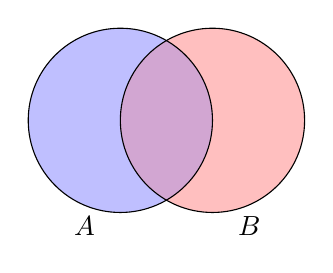
\begin{tikzpicture}[scale=0.9]
\fill[blue!25] \circA;
\fill[red!25] \circB;
\begin{scope}
\clip \circA;
\fill[violet!35] \circB;
\end{scope}
\draw \circA node[below left=1.1cm and 0.2cm]{$A$};
\draw \circB node[below right=1.1cm and 0.2cm]{$B$};
\end{tikzpicture}
\end{columns}
\end{frame}

\begin{frame}{Intersection of Sets}
\begin{columns}
\column{0.55\textwidth}
\begin{block}{Definition}
The intersection of two sets $A$ and $B$ is the set of all elements common to both.
$$A\cap B=\{x : x\in A \text{ and } x\in B\}$$
\end{block}
\begin{exampleblock}{Example: Image Dataset Filtering}
Let $D_1$ be the set of images containing cats, $D_2$ the set of images captured at night. Then $D=D_1\cap D_2$ = night-time cat images, usable to train/evaluate autonomous driving models.
\end{exampleblock}
\column{0.45\textwidth}
\centering
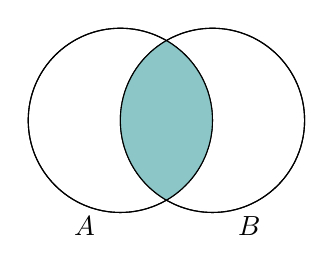
\begin{tikzpicture}[scale=0.9]
\draw \circA;
\draw \circB;
\begin{scope}
\clip \circA;
\clip \circB;
\fill[teal!45] (-2,-2) rectangle (4,2);
\end{scope}
\draw \circA node[below left=1.1cm and 0.2cm]{$A$};
\draw \circB node[below right=1.1cm and 0.2cm]{$B$};
\end{tikzpicture}
\end{columns}
\end{frame}

\begin{frame}{Set Difference}
\begin{columns}
\column{0.55\textwidth}
\begin{block}{Definition}
The set difference $A-B$ is the set of all elements that belong to $A$ but not to $B$.
$$A-B=\{x : x\in A \text{ and } x\notin B\}$$
\end{block}
\begin{exampleblock}{Example: Training Set Construction}
Let $D$ be the complete dataset and $T$ the test dataset. The training dataset is
$$\text{Train}=D-T$$
This removes all test samples from the complete dataset before training the model.
\end{exampleblock}
\column{0.45\textwidth}
\centering
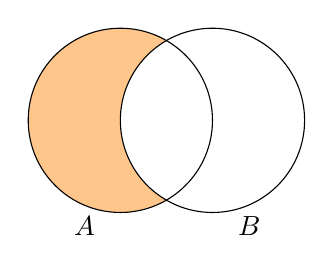
\begin{tikzpicture}[scale=0.9]
\begin{scope}
\clip \circA;
\fill[orange!45] (-2,-2) rectangle (4,2);
\end{scope}
\begin{scope}
\clip \circB;
\fill[white] (-2,-2) rectangle (4,2);
\end{scope}
\draw \circA node[below left=1.1cm and 0.2cm]{$A$};
\draw \circB node[below right=1.1cm and 0.2cm]{$B$};
\end{tikzpicture}
\end{columns}
\end{frame}

\begin{frame}{Symmetric Difference}
\begin{columns}
\column{0.55\textwidth}
\begin{block}{Definition}
The symmetric difference of $A$ and $B$ is the set of elements that belong to either $A$ or $B$, but not to both.
$$A\triangle B=(A-B)\cup(B-A)=(A\cup B)-(A\cap B)$$
\end{block}
\begin{exampleblock}{Example: Dataset Comparison in CV}
Let $D_1$ be images detected as cars by Model~1, $D_2$ images detected as cars by Model~2. $D_1\triangle D_2$ contains images classified as cars by only one of the two models -- useful for analyzing disagreements in model performance evaluation.
\end{exampleblock}
\column{0.45\textwidth}
\centering
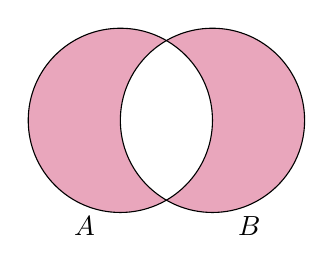
\begin{tikzpicture}[scale=0.9]
\begin{scope}
\clip \circA;
\fill[purple!35] (-2,-2) rectangle (4,2);
\end{scope}
\begin{scope}
\clip \circB;
\fill[purple!35] (-2,-2) rectangle (4,2);
\end{scope}
\begin{scope}
\clip \circA;
\clip \circB;
\fill[white] (-2,-2) rectangle (4,2);
\end{scope}
\draw \circA node[below left=1.1cm and 0.2cm]{$A$};
\draw \circB node[below right=1.1cm and 0.2cm]{$B$};
\end{tikzpicture}
\end{columns}
\end{frame}

\begin{frame}{Complement}
\small
\begin{columns}
\column{0.55\textwidth}
\begin{block}{Definition}
The complement of a set $A$ (denoted $A'$, $A^c$, or $U-A$) is the set of all elements in the universal set $U$ that are not in $A$.
$$A'=\{x : x\notin A \text{ and } x\in U\}$$
\end{block}
\begin{exampleblock}{Example: Dataset Partitioning}
Let $U=\{(x_i,y_i)\}_{i=1}^{N}$ be the complete labeled dataset, and $T\subseteq U$ the training dataset. The complement of $T$ is
$$T'=U-T$$
which represents all samples \emph{not} included in training (e.g. validation/test samples).
\end{exampleblock}
\column{0.45\textwidth}
\centering
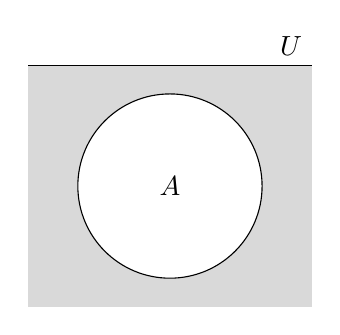
\begin{tikzpicture}[scale=0.9]
\draw (-2,-1.7) rectangle (2,1.7);
\fill[gray!30] (-2,-1.7) rectangle (2,1.7);
\begin{scope}
\clip (0,0) circle (1.3);
\fill[white] (-2,-2) rectangle (2,2);
\end{scope}
\draw (0,0) circle (1.3) node{$A$};
\node[above left] at (2,1.7) {$U$};
\end{tikzpicture}
\end{columns}
\end{frame}

\begin{frame}{Cartesian Product}
\begin{block}{Definition}
The Cartesian product of two sets $A$ and $B$ is the set of all ordered pairs $(a,b)$ where $a\in A$ and $b\in B$.
$$A\times B=\{(x,y) : x\in A \text{ and } y\in B\}, \qquad |A|=m,\ |B|=n \implies |A\times B|=mn$$
\end{block}
\begin{exampleblock}{Example: Feature Vectors and Class Labels}
Let $X=\{x_1,x_2,\dots,x_n\}$ be the set of input feature vectors and $Y=\{y_1,y_2,\dots,y_k\}$ the set of class labels. Then
$$X\times Y=\{(x,y) \mid x\in X,\ y\in Y\}$$
represents the set of all possible (input, label) pairings.
\end{exampleblock}
\end{frame}

% ===========================================================
\section{Inclusion--Exclusion Principle}
% ===========================================================

\begin{frame}{Inclusion--Exclusion Principle}
\begin{block}{Definition}
A counting technique used to determine the number of elements in the union of two or more sets, by adding the sizes of the sets and subtracting the sizes of their intersections, to avoid double counting.
\end{block}

\begin{columns}
\column{0.55\textwidth}
\textbf{Two sets:}
$$|A\cup B|=|A|+|B|-|A\cap B|$$

\textbf{Three sets:}
\begin{align*}
|A\cup B\cup C| = {}& |A|+|B|+|C| \\
& -|A\cap B|-|A\cap C|-|B\cap C| \\
& +|A\cap B\cap C|
\end{align*}

\column{0.45\textwidth}
\centering
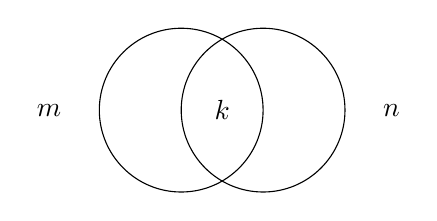
\begin{tikzpicture}[scale=0.8]
\draw \circA node[left=1.4cm]{$m$};
\draw \circB node[right=1.4cm]{$n$};
\node at (0.65,0) {$k$};
\end{tikzpicture}
$$|A\cup B| = m+k+n+k-k = m+k+n$$
\end{columns}
\end{frame}

\begin{frame}{Inclusion--Exclusion: General Form \& Example}
\begin{block}{General Form}
$$\left|\bigcup_{i=1}^{n}A_i\right| = \sum_i |A_i| - \sum_{i<j}|A_i\cap A_j| + \sum_{i<j<k}|A_i\cap A_j \cap A_k| - \cdots + (-1)^{n+1}\left|\bigcap_{i=1}^{n}A_i\right|$$
\end{block}
\begin{exampleblock}{Example: Market-Basket Transactions}
Let $T_1$ = set of transactions containing Milk, $T_2$ = set of transactions containing Bread. The total number of transactions containing Milk \emph{or} Bread is
$$|T_1\cup T_2| = |T_1|+|T_2|-|T_1\cap T_2|$$
\end{exampleblock}
\end{frame}

% ===========================================================
\section{Partially Ordered Sets \& Hasse Diagrams}
% ===========================================================

\begin{frame}{Partially Ordered Set (Poset)}
\begin{block}{Definition}
A relation $R$ on a set $A$ is a \textbf{partial order} if it is:
\begin{itemize}
\item \textbf{Reflexive} -- $aRa$ for all $a\in A$
\item \textbf{Antisymmetric} -- $aRb$ and $bRa \implies a=b$
\item \textbf{Transitive} -- $aRb$ and $bRc \implies aRc$
\end{itemize}
The set $A$ together with $R$ is called a \textbf{partially ordered set} (poset).
\end{block}
\begin{exampleblock}{Example 1: $\le$ on $A=\{1,2,3,4,5\}$}
$aRb \iff a\le b$
$$R=\{(1,1),(1,2),(1,3),(1,4),(1,5),(2,2),(2,3),(2,4),(2,5),$$
$$(3,3),(3,4),(3,5),(4,4),(4,5),(5,5)\}$$
\end{exampleblock}
\end{frame}

\begin{frame}{Hasse Diagram: Chain $\{1,2,3,4,5\}$}
\begin{block}{Idea}
A \textbf{Hasse diagram} is a simplified drawing of a poset: reflexive loops and transitive edges are omitted, and $a<b$ is drawn with $b$ higher than $a$, connected by an edge only if there is no element strictly between them (covering relation).
\end{block}
\centering
\begin{tikzpicture}[node distance=0.9cm]
\node (n1) at (0,0) {1};
\node (n2) at (0,1) {2};
\node (n3) at (0,2) {3};
\node (n4) at (0,3) {4};
\node (n5) at (0,4) {5};
\draw (n1)--(n2)--(n3)--(n4)--(n5);
\end{tikzpicture}
\end{frame}

\begin{frame}{Poset Example 2: Power Set of $\{1,2,3\}$ under $\subseteq$}
\begin{exampleblock}{Setup}
$A=\{1,2,3\}$, \quad $S=\mathcal{P}(A)=\{S_0,S_1,\dots,S_7\}$ where
$$S_0=\varnothing,\ S_1=\{1\},\ S_2=\{2\},\ S_3=\{3\},\ S_4=\{1,2\},\ S_5=\{1,3\},\ S_6=\{2,3\},\ S_7=\{1,2,3\}$$
\end{exampleblock}
\begin{block}{Relation}
$$S_iRS_j \iff S_i\subseteq S_j$$
This relation is reflexive, antisymmetric and transitive $\implies (\mathcal{P}(A),\subseteq)$ is a poset.
\end{block}
\end{frame}

\begin{frame}{Hasse Diagram: $(\mathcal{P}(\{1,2,3\}),\subseteq)$}
\centering
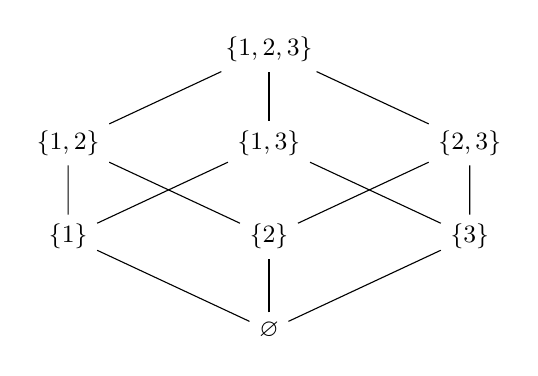
\begin{tikzpicture}[scale=0.85, every node/.style={font=\small}]
% level 0
\node (e) at (0,0) {$\varnothing$};
% level 1
\node (a) at (-3,1.4) {$\{1\}$};
\node (b) at (0,1.4) {$\{2\}$};
\node (c) at (3,1.4) {$\{3\}$};
% level 2
\node (ab) at (-3,2.8) {$\{1,2\}$};
\node (ac) at (0,2.8) {$\{1,3\}$};
\node (bc) at (3,2.8) {$\{2,3\}$};
% level 3
\node (abc) at (0,4.2) {$\{1,2,3\}$};

\draw (e)--(a); \draw (e)--(b); \draw (e)--(c);
\draw (a)--(ab); \draw (a)--(ac);
\draw (b)--(ab); \draw (b)--(bc);
\draw (c)--(ac); \draw (c)--(bc);
\draw (ab)--(abc); \draw (ac)--(abc); \draw (bc)--(abc);
\end{tikzpicture}
\end{frame}

\begin{frame}
\centering
\Huge Thank You
\end{frame}

\end{document}